\chapter{State of the Art}
\label{chapter: State of the Art}

%%% SECTION

This chapter's  major aim  is to revise the existing scientific literature on the skin lesions classification, which represents a fundamental part of the research work. The section has been presented in chronological order, which allows us to see the evolution in this field of medicine over time. The following chapter is structured into three sections: First, the architectures that were initially used based on Machine Learning (ML), second, the emergence of Neural Networks using image classification, and finally, the latest trends in this kind of architecture. In each section, the advances are introduced, identifying characteristics and limitations.

\section{Feature Extraction in Machine Learning}
Since last century decade, research into expert systems for image processing in medicine to support diagnosis has been in progress  \cite{beuscart_expert_1997}, \cite{chan_expert_1996}.  We could already find diagnostic work based on neural networks \cite{wells_medical_1998} at the end of the 20th century, nevertheless, the trend in research was using Machine Learning (ML) algorithms for image classification \cite{dreiseitl_comparison_2001}, \cite{dreiseitl_classifying_2000}. Thus, during the first years of the 21st century, research efforts were focused on improving the performance of ML algorithms by adding a \textbf{previous layer feature selection} \cite{lee_machine_2009}. An example of it can be found in this text \cite{garnavi_computer-aided_2012}, where the authors performed a benchmark with machine learning classifiers, measuring the impact of using a preprocess to extract texture, contour delineation and geometric properties of the melanoma lesion before moving to the classification stage.  They conclude that the three features used make the classifier perform better, with texture being the dominant feature to improve the accuracy metric. Finding feature extraction allows sample discrimination and classification which is ML algorithms' main problem when processing medical images, including dermoscopic images. In this medicine area, the asymmetry, border, colours and dermoscopic rule (also known as \textbf{ABCD rule} in dermatology) or the colour, architecture, symmetry and homogeneity (\textbf{CASH rule}) is common to support the classification \cite{lee_machine_2009}. Concerning this point, in 2012 \cite{6263297} we could find a research document where a \textbf{complete feature extractor} was built with a preprocessing stage for lesion boundary delimitation, the symmetry presented two axes, the lesion geometry and as well as its texture.  The feature output extractor  fed four ML classifiers (Support Vector Machine (SVM), random forest, logistic model tree and hidden naive Bayes) with outstanding results. In 2014, the k-means algorithm used for sample separation into colours, together with a logistic regression already achieved a sensitivity of 62\% and a specificity of 76\% \cite{6803866}. Meanwhile, in 2015 \cite{abuzaghleh_noninvasive_2015}, the application of  SVM in cascade configuration together with a filter for hair detection, a Gaussian low-pass filtering on each of the channels allows higher accuracy, approaching 98 \%.

\section{The Image Processing Evolution with Neural Networks}

As we have presented above, research in image processing using neural networks dates back to the end of the 20th century, it is from the first decade of the 21st century that developments based on this technology begin to emerge strongly, though. This is due to the use of graphics processing units (GPUs) to compute the calculations, subsequently, tensor processing units (TPUs) were added, together with the provision of large labelled data sets and the commitment to innovate by large technology companies and institutions. Thus, in 2011, the famous paper "\textit{Building High-level Features Using Large Scale Unsupervised Learning}" \cite{le_building_2012} by Google engineers established a turning point in image processing by using neural networks for large-scale unsupervised learning on 31,000 images. Unlike the ML models seen above, neural networks belong to the group of unsupervised classifiers, where the system identifies the main features, without relying on manual supervision \cite{Le2011BuildingHF}. In contrast to the previous trend in ML, which added complexity to models by focusing on the feature extraction layer, with neural networks, the\textbf{ network learns to extract the most relevant patterns from the image by itself}.

Within the set of types of neural networks, we find that there is a group with direct applications in image processing. We refer to \textbf{convolutional neural networks} (CNN) \cite{shiri_comprehensive_nodate} \cite{chen_review_2021}, which extract increasingly complex patterns as we go deeper into the layers of the network, increasing the level of abstraction of the object concerning the image. In this way, the network learns features and patterns that allow it to distinguish the object through training, accurately detecting those same patterns in other images not used during that process time. Each layer of the CNN neural network acts as a filter that detects a certain pattern in the image. Therefore, it is easy to think that increasing the number of layers will increase the model's reliability. Nevertheless, this action will also increase the number of parameters to train and so, will increase the training time of these models. This philosophy gives birth to the concept of \textbf{Deep Learning }(DL) \cite{noauthor_what_nodate} as a subfield within the area of ML.

\begin{figure}[ht]
    \begin{center}
        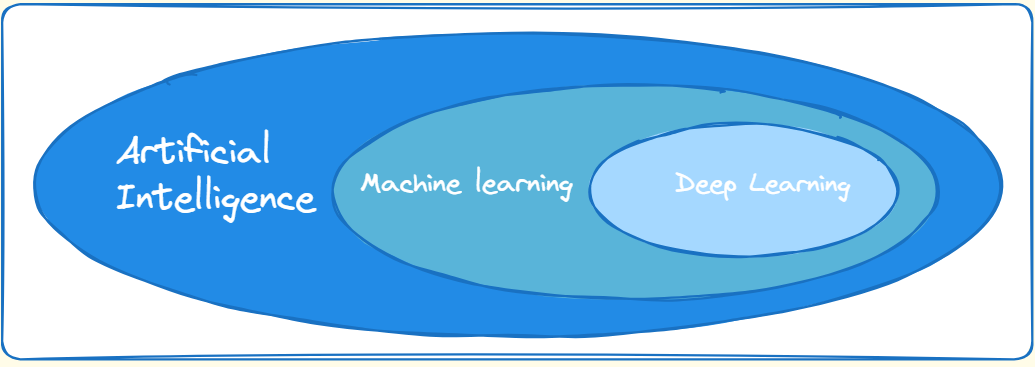
\includegraphics[scale=0.60]{images/AI_Group.png}
        \caption{Relationships among the subgroups that make up artificial intelligence.}
    \label{fig:IA Subgroup}    
    \end{center}
\end{figure}


\section{Advances in Image Classification for Dermatology: Overcoming Challenges with Deep Learning and  Pre-processing Images}

The contemporary trend is to use  \textbf{intense networks} for image classification in the medical field, specifically in dermatology. However, incorporating more and more layers, results in an increase in the parameter numbers causing a possible network's degradation \cite{roy_effects_2023}. To overcome the degradation problem in this type of network, a technique used is \textbf{residual learning}, with a Fully Convolutional 
Residual Network (FCRN). It can be seen in  \cite{7792699}, where intense neural networks have used more than 50 layers with an initial image segmentation process before moving on to the classification stage.  This type of network, \cite{laina_deeper_2016} is based on the idea of allowing neural network layers to learn the differences between the input and output, also known as residual learning. This is achieved by introducing hops in one or more network layers, which makes possible the convergence in deep networks avoiding exploding or vanishing gradients \cite{wong_what_2021}.

In order to have a better model accuracy without increasing the number of layers too much,  it is necessary to go back to the idea of implementing a pre-processing layer to extract the main features before the classification. Thus in this work \cite{thamizhamuthu_deep_2023}, a k-means machine learning algorithm is employed at the pre-processing stage, which purpose is to segment the pixels by colour. In this sense, these layers aim to isolate the lesioned region from the rest of the skin, and then go on to a feature extraction stage to determine the colour, the information intensity of each channel and the lesion pattern using different algorithms. The result is then passed to a feature selection stage that uses the statistical \textit{t-test} to decide the feature's importance. These are classified by category to determine the image's dominant feature set, and the classified features feed a deep neural network. The results obtained are significant, reaching 99 \% Accuracy with 98.33 \% sensitivity. 

Another trend used in the last decade for the specific case of skin photo processing is the incorporation of a filter before the convolutional network  removes the noise caused by hair in dermoscopic images.\cite{talavera-martinez_hair_2021}, \cite{bardou_hair_2022}, \cite{kaur_hairlines_2022}.

One of the problems facing neural network training is the need to process an extensive set of quality data. To minimise the impact of having poor data and improving the time used during this part, the \textbf{transfer learning} technique has been implemented in neural network architectures over the last decade \cite{rodrigues_new_2020}, \cite{wall_deep_2020}, \cite{abbes_deep_2021}, \cite{georgakopoulos_detection_2017}. The concept behind this technique lies underneath taking advantage of the knowledge acquisition process for other long and specific neural networks. Instead of training a model from scratch for a new task, transfer learning uses a pre-trained model from a previous task as a starting point. This pre-trained model has already learned useful features and data patterns that can be applied to the new task, which speeds up the training process and can result in better performance. 

Another problem commonly faced by CNNs is the overfitting risk caused by limited data sources. It is common in these cases to incorporate \textbf{data augmentation} techniques, so as to introduce variability and increase the data quantity \cite{shorten_survey_2019}. These techniques apply transformation methods to the image such as rotation, translation, flipping, zoom or noise injection. 

